\documentclass[11pt,openright,a4paper]{article}
\usepackage{fancyhdr}
\usepackage{datetime}
\usepackage[left=25mm,right=25mm,top=35mm,bottom=35mm,footskip=0.5in]{geometry}
% %%
%% Package includes to provide the basic style
%%
\usepackage{harvard}    % Uses harvard style referencing
\usepackage{graphicx}   % Permits import of various graphics formats
\usepackage{hyperref}   % Provides hyperlinks to sections automatically
\usepackage{pdflscape}  % Provides landscape mode for end code listings
\usepackage{multicol}   % Provides ability to split output into columns
\usepackage{listings}   % Provides styled code listings
\usepackage{titlesec}
\usepackage[margin=35mm,footskip=0.5in]{geometry}
\usepackage{tabularx}
\usepackage{tabulary}
\usepackage{multirow}
\usepackage{color}
\usepackage[table]{xcolor}
\usepackage{caption, subcaption}
\usepackage{amssymb, amsmath, empheq}
\lstset{language=Python}
\usepackage{array}
\usepackage{longtable}
\usepackage{subfiles}
\usepackage{float}
\usepackage{longtable}

\graphicspath{ {images/} {lit_review/images/} {images/tech/} {images/methodology/} {images/results/} }
% \numberwithin{equation}{chapter}

\let\subsectionautorefname\sectionautorefname
\let\subsubsectionautorefname\sectionautorefname

% % set margin
% \geometry{
%   a4paper,
%   top=25mm,
%   bottom=35mm
% }

%%
%% Set some page size changes from the standard article class
%%
\usepackage{calc}
\setlength{\parskip}{6pt}
\setlength{\parindent}{0pt}
\addtolength{\hoffset}{0.5cm}
\addtolength{\textwidth}{0.5cm}

% set section depth
\setcounter{tocdepth}{4}
\setcounter{secnumdepth}{5}

% set chapter format
%\titleformat{\chapter}[hang]{\LARGE\bfseries}{\thechapter\hspace{20pt}}{0pt}{\LARGE\bfseries}
%\titlespacing{\chapter}{0pt}{0pt}{5pt}

%%
%% Format definitions for the style
%%
\bibliographystyle{agsm}  %{alpha}
\citationstyle{dcu}
\pagestyle{headings}
\fussy


%%
%% Definitions to provide layout in the dissertation title pages
%%
\newenvironment{spaced}[1]
  {\begin{minipage}[c]{\textwidth}\vspace{#1}}
  {\end{minipage}}


\newenvironment{centrespaced}[2]
  {\begin{center}\begin{minipage}[c]{#1}\vspace{#2}}
  {\end{minipage}\end{center}}


%%
%% New column header command
%% 
\newcolumntype{Z}{ >{\centering\arraybackslash}X }
\newcolumntype{M}[1]{ >{\centering\arraybackslash}m{#1}}


% declaration
\newcommand{\declaration}[2]{
  \thispagestyle{empty}
  \begin{spaced}{4em}
    \begin{center}
      \LARGE\textbf{#1}
    \end{center}
  \end{spaced}
  \begin{spaced}{3em}
    \begin{center}
      Submitted by: #2
    \end{center}
  \end{spaced}
  \begin{spaced}{5em}
    \section*{COPYRIGHT}

    Attention is drawn to the fact that copyright of this dissertation rests
    with its author. The Intellectual Property Rights of the products
    produced as part of the project belong to the author unless otherwise specified
    below, in accordance with the University of Bath's policy on intellectual property 
   (see http://www.bath.ac.uk/ordinances/22.pdf).

    This copy of the dissertation has been supplied on condition that anyone
    who consults it is understood to recognise that its copyright rests with its
    author and that no quotation from the dissertation and no information
    derived from it may be published without the prior written consent of
    the author. \\ \\

    \section*{DECLARATION}
    This dissertation is submitted to the University of Bath in accordance
    with the requirements of the degree of Bachelor of Science in the
    Department of Computer Science. No portion of the work in this dissertation
    has been submitted in support of an application for any other degree
    or qualification of this or any other university or institution of learning.
    Except where specifically acknowledged, it is the work of the author.
  \end{spaced}

  \begin{spaced}{5em}
    Signed:
  \end{spaced}
  }


% consultation
\newcommand{\consultation}[1]{%
\thispagestyle{empty}
\begin{centrespaced}{0.8\textwidth}{0.4\textheight}
\ifnum #1 = 0
This dissertation may be made available for consultation within the
University Library and may be photocopied or lent to other libraries
for the purposes of consultation.
\else
This dissertation may not be consulted, photocopied or lent to other
libraries without the permission of the author for #1 
\ifnum #1 = 1
year
\else
years
\fi
from the date of submission of the dissertation.
\fi
\vspace{4em}

Signed:
\end{centrespaced}
}

%%
%% END OF DEFINITIONS
%%


\usepackage{amsmath}
\usepackage{hyperref}
\usepackage{amsbsy}
\usepackage{graphicx}
\usepackage{float}

\usepackage[english]{babel}
\usepackage[backend=bibtex,sorting=none,style=ieee]{biblatex}
\bibliography{task2bib}

\graphicspath{ {images/} }
\usepackage{graphicx}

% header
\pagestyle{fancy}
\fancyhf{}
\lhead{CM50426 Machine Learning \& AI \\ Alan Lau}
\rhead{Task 2 \\ Semester 1, 2016-17}
\cfoot{\thepage}

\setlength{\parindent}{0em}
\setlength{\parskip}{1em}
\numberwithin{equation}{section}

\abovedisplayskip=12pt plus 3pt minus 9pt
\abovedisplayshortskip=0pt plus 3pt
\belowdisplayskip=12pt plus 3pt minus 9pt
\belowdisplayshortskip=7pt plus 3pt minus 4pt

\usepackage[font=small,labelfont=bf]{caption}


% define a macro \Autoref to allow multiple references to be passed to \autoref
\newcommand\Autoref[1]{\@first@ref#1,@}
\def\@throw@dot#1.#2@{#1}% discard everything after the dot
\def\@set@refname#1{%    % set \@refname to autoefname+s using \getrefbykeydefault
    \edef\@tmp{\getrefbykeydefault{#1}{anchor}{}}%
    \def\@refname{\@nameuse{\expandafter\@throw@dot\@tmp.@autorefname}s}%
}
\def\@first@ref#1,#2{%
  \ifx#2@\autoref{#1}\let\@nextref\@gobble% only one ref, revert to normal \autoref
  \else%
    \@set@refname{#1}%  set \@refname to autoref name
    \@refname~\ref{#1}% add autoefname and first reference
    \let\@nextref\@next@ref% push processing to \@next@ref
  \fi%
  \@nextref#2%
}
\def\@next@ref#1,#2{%
   \ifx#2@ and~\ref{#1}\let\@nextref\@gobble% at end: print and+\ref and stop
   \else, \ref{#1}% print  ,+\ref and continue
   \fi%
   \@nextref#2%
}


\begin{document}

% - Differences between ML, MAP and Bayesian
    % - suitability, pros and cons
    % - how to pick a model to use based on the data
% - What is meant by overfitting in non-linear
% - How to initialise the models

% - Why does the method work, and when
% - How efficient is the method (accuracy VS computational expensiveness)
% - Compare with other methods
% - How could I improve it

%%%%%%%%%%%%%
\section{Introduction} \label{sec:intro}
%%%%%%%%%%%%%
Regression is a supervised machine learning method that aims to estimate a univariate continuous target ($y$) or the world state ($w$), given some $D$-dimensional observed measures as the input ({$\mathbf{x}$}), so that we can use this to predict some new input. For example, one may want to predict the price of a house given input information of size, location, number of bedrooms and age of the house. Visually, this is done through fitting a line through the data.

\begin{equation} \label{eq:base-assign}
    \begin{aligned}
        \mathbf{x}_i &\leftarrow \left [ 1 \quad \mathbf{x}_{i}^{T}  \right ] \\
        \mathbf{\phi} &\leftarrow \left [ \phi_0 \quad \boldsymbol\phi^T \right ]^T
    \end{aligned}
\end{equation}

\begin{equation} \label{eq:base}
    Pr \left( w_i | \mathbf{x}_i, \boldsymbol\theta \right) = \text{Norm}_{w_i} \left [ \boldsymbol\phi^T \mathbf{x}_i, \sigma^2 \right ]
\end{equation}

The linear regression model is a normal distribution using a linear equation as the $\boldsymbol\mu$ input. The model is defined as below in \autoref{eq:base}. Note that we have done the assignments in \autoref{eq:base-assign} to make the notation neater and easier to compute, by combining the gradients $\boldsymbol\phi$ with the $y$-intercept.


\begin{equation} \label{eq:base-all}
    Pr \left( \mathbf{w} | \mathbf{X} \right) = 
    \text{Norm}_w \left [ \mathbf{X}^T \phi, \; \sigma^2\mathbf{I} \right ]
\end{equation}

Hence, the likelihood for the whole input dataset is given by \autoref{eq:base-all}, where $\mathbf{X} = [ \mathbf{x}_1,...,\mathbf{x}_I ]$ is the input vector, $\mathbf{w} = [w_1,...,w_I]^T$ is the target over the whole dataset, and I is the $D$*$D$ identity matrix.

We are now going to look at three approaches for estimating the parameters, $\boldsymbol{\phi}$ and $\boldsymbol{\sigma}^2$.


%%%%%%%%%%%%
\section{Linear Regression} \label{sec:approaches}
%%%%%%%%%%%%

\subsection{Maximum Likelihood (ML)} \label{ssec:apporaches-ml}

\begin{equation} \label{eq:ml-argmax}
    \begin{aligned}
        \hat{\boldsymbol\theta} &=
            \mathrm{argmax}_{\theta}
                \left [
                    \log{\left [ Pr \left ( \mathbf{w} | \mathbf{X}, \boldsymbol\theta \right ) \right ]}
                \right ]
        \\
        \hat{\boldsymbol\theta}, \hat{\sigma}^2 &=
            \mathrm{argmax}_{\boldsymbol\theta, \sigma^2}
            \left [
                - \frac{ I \log{\left ( 2 \pi  \right )} }{2}
                - \frac{ I \log{\left ( \sigma^2  \right )} }{2}
                - \frac{\left ( \mathbf{w} - \mathbf{X}^T\boldsymbol\phi \right )^T  \left ( \mathbf{w} - \mathbf{X}^T\boldsymbol\phi \right )}
                       {2\sigma^2}
            \right ]
    \end{aligned}
\end{equation}

Here, we aim to find the parameters, $\boldsymbol\theta$, by maximising the likelihood. To facilitate computation, we maximise the log likelihood. By expanding, we get \autoref{eq:ml-argmax}. Differentiating the \autoref{eq:ml-argmax} with repsect to the two variables separately and equating each to zero, we get the following equations, giving us the ML estimates for the parameters:

\begin{equation} \label{eq:ml-params}
    \begin{aligned}
        \hat{\boldsymbol\phi} &=
            \left ( \mathbf{XX}^T  \right ) \mathbf{Xw}
        \\
        \hat{\sigma}^2 &=
            \frac{\left ( \mathbf{w} - \mathbf{X}^T\boldsymbol\phi \right )^T  \left ( \mathbf{w} - \mathbf{X}^T\boldsymbol\phi \right )}{I}
    \end{aligned}
\end{equation}

\begin{figure}[H]
  \centering
  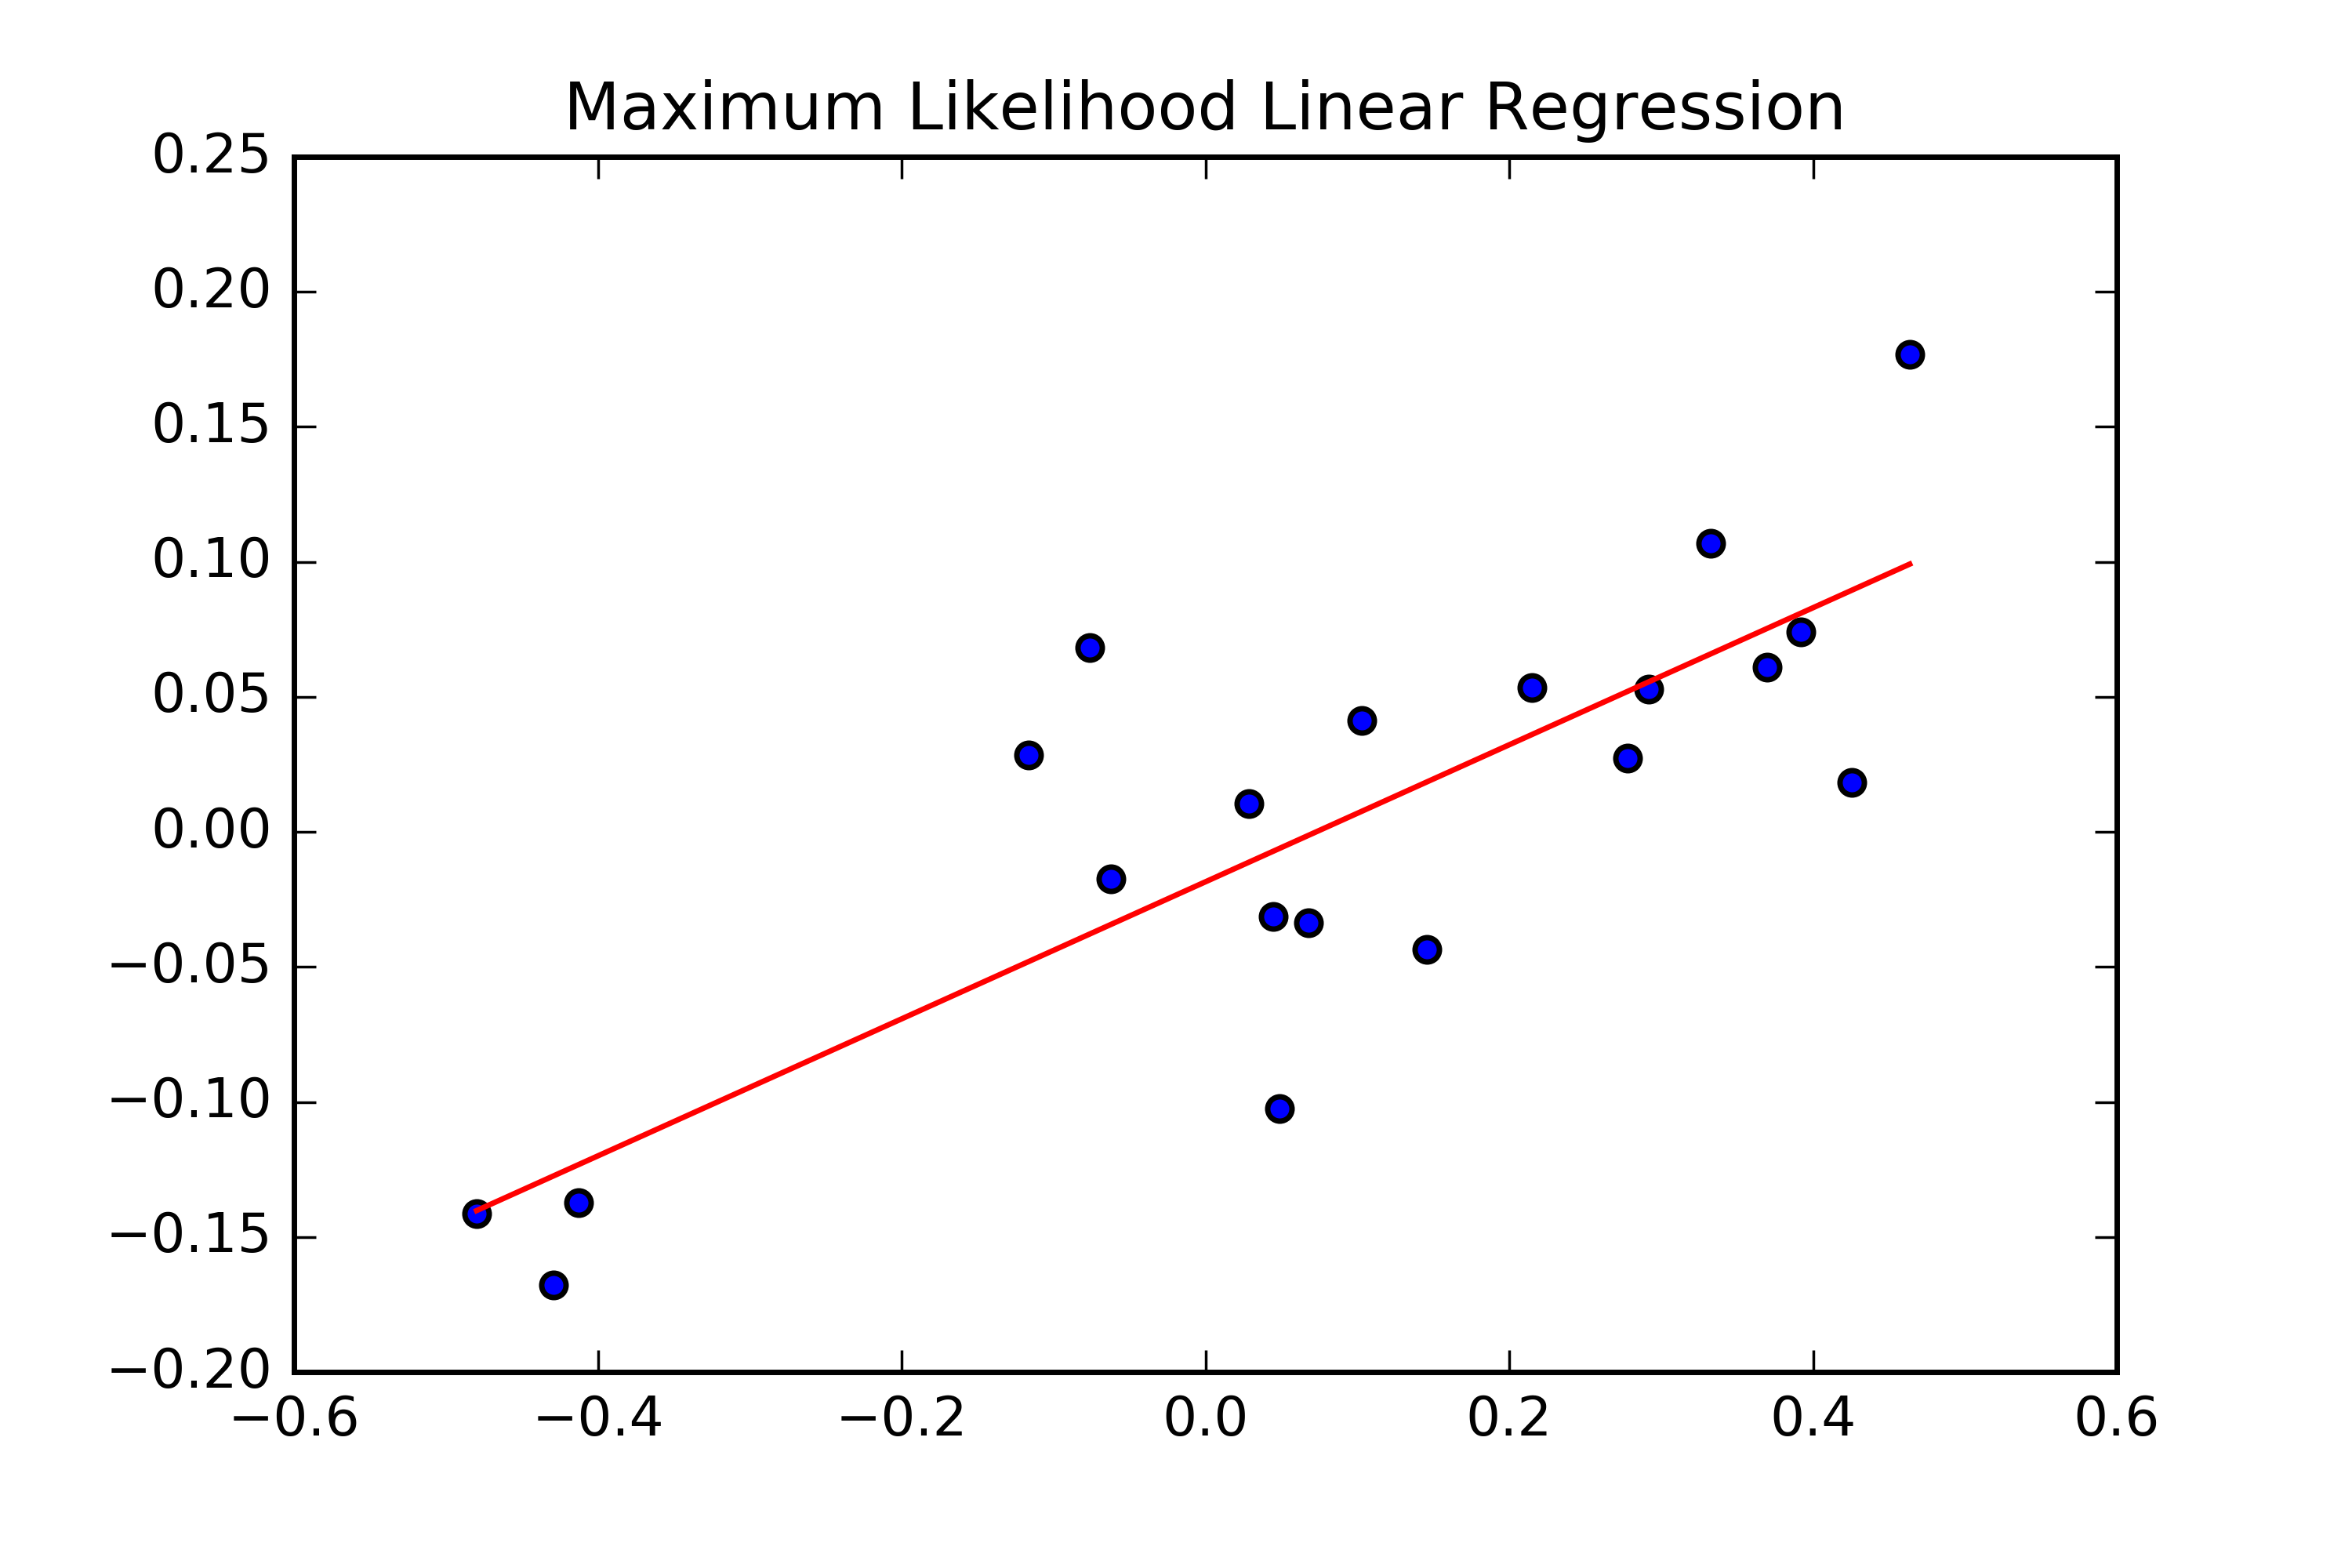
\includegraphics[width=0.7\textwidth]{lin-ml}
    \caption{Linear regression with Maximum Likelihood parameter estimation.}
  \label{fig:lin-ml}
\end{figure}

\subsection{Bayesian} \label{ssec:approaches-bayesian}

\subsubsection{Background}
\begin{equation} \label{eq:bayes}
    Pr \left ( \boldsymbol\phi | \mathbf{X}, \mathbf{w} \right ) =
        \frac{Pr \left (\mathbf{w} | \mathbf{X}, \boldsymbol\phi \right ) \; Pr \left ( \boldsymbol\phi  \right )}
             {Pr \left ( \mathbf{w} | \mathbf{X} \right )}
\end{equation}

Rather than calculating the parameter than maximises the likelihood, we calculate the probability distribution over all possible values of $\boldsymbol\phi$. We consider a prior with zero mean and spherical covariance as $\boldsymbol\phi$ is multivariate and continuous, and the likelihood as illustrated with \autoref{eq:base-all}.

By observing the Bayes' Rule in \autoref{eq:bayes} and combining the normal distributions of the likelihood, prior and evidence, we obtain \autoref{eq:posterior} to compute the posterior distribution. Note that a $D \times D$ identity matrix $\mathbf{I}_D$ is used here.

\begin{equation} \label{eq:posterior}
    Pr \left ( \boldsymbol\phi | \mathbf{X}, \mathbf{w} \right ) =
        \text{Norm}_{\phi} 
            \left [ \frac{1}{\sigma^2} \mathbf{A^{-1} X w} , \; \mathbf{A}^{-1} \right ]
\end{equation}

where

\begin{equation} \label{eq:bayes-a}
    \mathbf{A} = \frac{1}{\sigma^2} \mathbf{X X}^T + \frac{1}{\sigma_p^2}\mathbf{I}_D
\end{equation}

\subsubsection{Computing Large Inverses}

\begin{equation} \label{eq:inv-a}
    \begin{aligned}
        \mathbf{A}^{-1} &=
        \left ( \frac{1}{\sigma^2} \mathbf{X X}^T + \frac{1}{\sigma_p^2}\mathbf{I}_D \right )^{-1}
        \\
        &=  \sigma_p^2 \mathbf{I}_D -
            \sigma_p^2 \mathbf{X}
            \left ( \mathbf{X}^T\mathbf{X} + 
                \frac{\sigma^2}{\sigma_p^2} \mathbf{I}_I \right )^{-1}
            \mathbf{X}^T
    \end{aligned}
\end{equation}

\autoref{eq:bayes-a} becomes a large matrix at high dimensions, which poses a problem when the inverse is required. By applying the matrix inverse lemma as shown in \autoref{eq:inv-a}, we can make the calculation less computationally demanding when the dimension of each input datapoint is large, as the dimensions of the identitiy matrix used has now become $I \times I$, instead of $D \times D$.

\subsubsection{Inferences}

\begin{equation} \label{eq:inference}
    \begin{aligned}
        Pr \left ( w^* | \mathbf{x}^*, \mathbf{X}, \mathbf{w}  \right )
        &=
        \int Pr \left ( w^*|\mathbf{x}^*, \mathbf{\sigma^2} \right )
             Pr \left ( \boldsymbol\phi | \mathbf{X}, \mathbf{w} \right ) 
        \; d \boldsymbol\phi
        \\
        &= \text{Norm}_{w^*} \left [
           \frac{1}{\sigma^2} \mathbf{x}^{*T} \mathbf{A}^{-1} \mathbf{X w}, \;
           \mathbf{x}^{*T} \mathbf{A^{-1}x}^* + \sigma^2
           \right ]
    \end{aligned}
\end{equation}

We can then use the posterior distribution result to perform inferences. Here, we are calculating the predictive distribution over the world state $w^*$ given the original observed vector $\mathbf{X}$ and target vector $\mathbf{w}$, and a new observed data vector $\mathbf{x}^*$. In other words, our goal is to show a distribution of how probable an unseen datapoint has some target labels, which we expect our model to be less confident as it gets further away from the mean of the dataset, i.e. the most densely packed areas.

As seen in \autoref{eq:inference}, we use the posterior distribution (\autoref{eq:posterior}) as weight to the predictive distribution. Through marginalising $\boldsymbol\phi$, we obtain the predictive distribution, which is a normal distribution. 

Unlike ML or MAP, a Bayesian approach tries to be as fair as possible by giving a distribution rather than a point-wise prediction. It also acts act more intuitively like how we would approach a real-world problem. However, the inference is too difficult to be computed, even with the matrix trick illustrated in \autoref{eq:inv-a}. Approximate inferences is therefore used. 

\subsection{Maximum A Priori (MAP)}

\begin{equation} \label{eq:map-phi}
    \begin{aligned}
        \frac{1}{2\sigma^2}
            \left ( 2 \mathbf{Xw} - 2 \mathbf{XX}^T \boldsymbol{\phi} \right ) -
            \frac{1}{\sigma_p^2} \boldsymbol\phi &= 0
        \\
        \left ( \mathbf{Xw} - \mathbf{XX}^T\boldsymbol\phi \right ) -
            \frac{\sigma^2}{\sigma_p^2}\boldsymbol\phi &= 0
        \\
        \mathbf{Xw} - \left ( \mathbf{XX}^T + \frac{\sigma^2}{\sigma_p^2} \mathbf{I}  \right ) \boldsymbol\phi &= 0
        \\
        \hat{\boldsymbol\phi} &= 
            \left ( \mathbf{XX}^T + \frac{\sigma^2}{\sigma_p^2} \mathbf{I} \right )^{-1} \mathbf{Xw}
    \end{aligned}
\end{equation}

With MAP, we take into account the prior in order to estimate the parameters. In other words, we aim to choose parameters that maximises the posterior probability. For $\boldsymbol\phi$, we have a closed-form solution which is derived by marginalising $\phi$ in \autoref{eq:bayes}. By equating the derivative to zero, we have our estimated $\boldsymbol\phi$, as shown in \autoref{eq:map-phi}.

The covariance $\sigma^2$ can be simply done through ML as shown in \autoref{eq:ml-params} for simplicity, as it is done for this piece of coursework, but it could also be performed by using a non-linear optimisation technique to maximise the posterior simultaneously for both parameters such as Newton's method.


\begin{figure}[H]
  \centering
  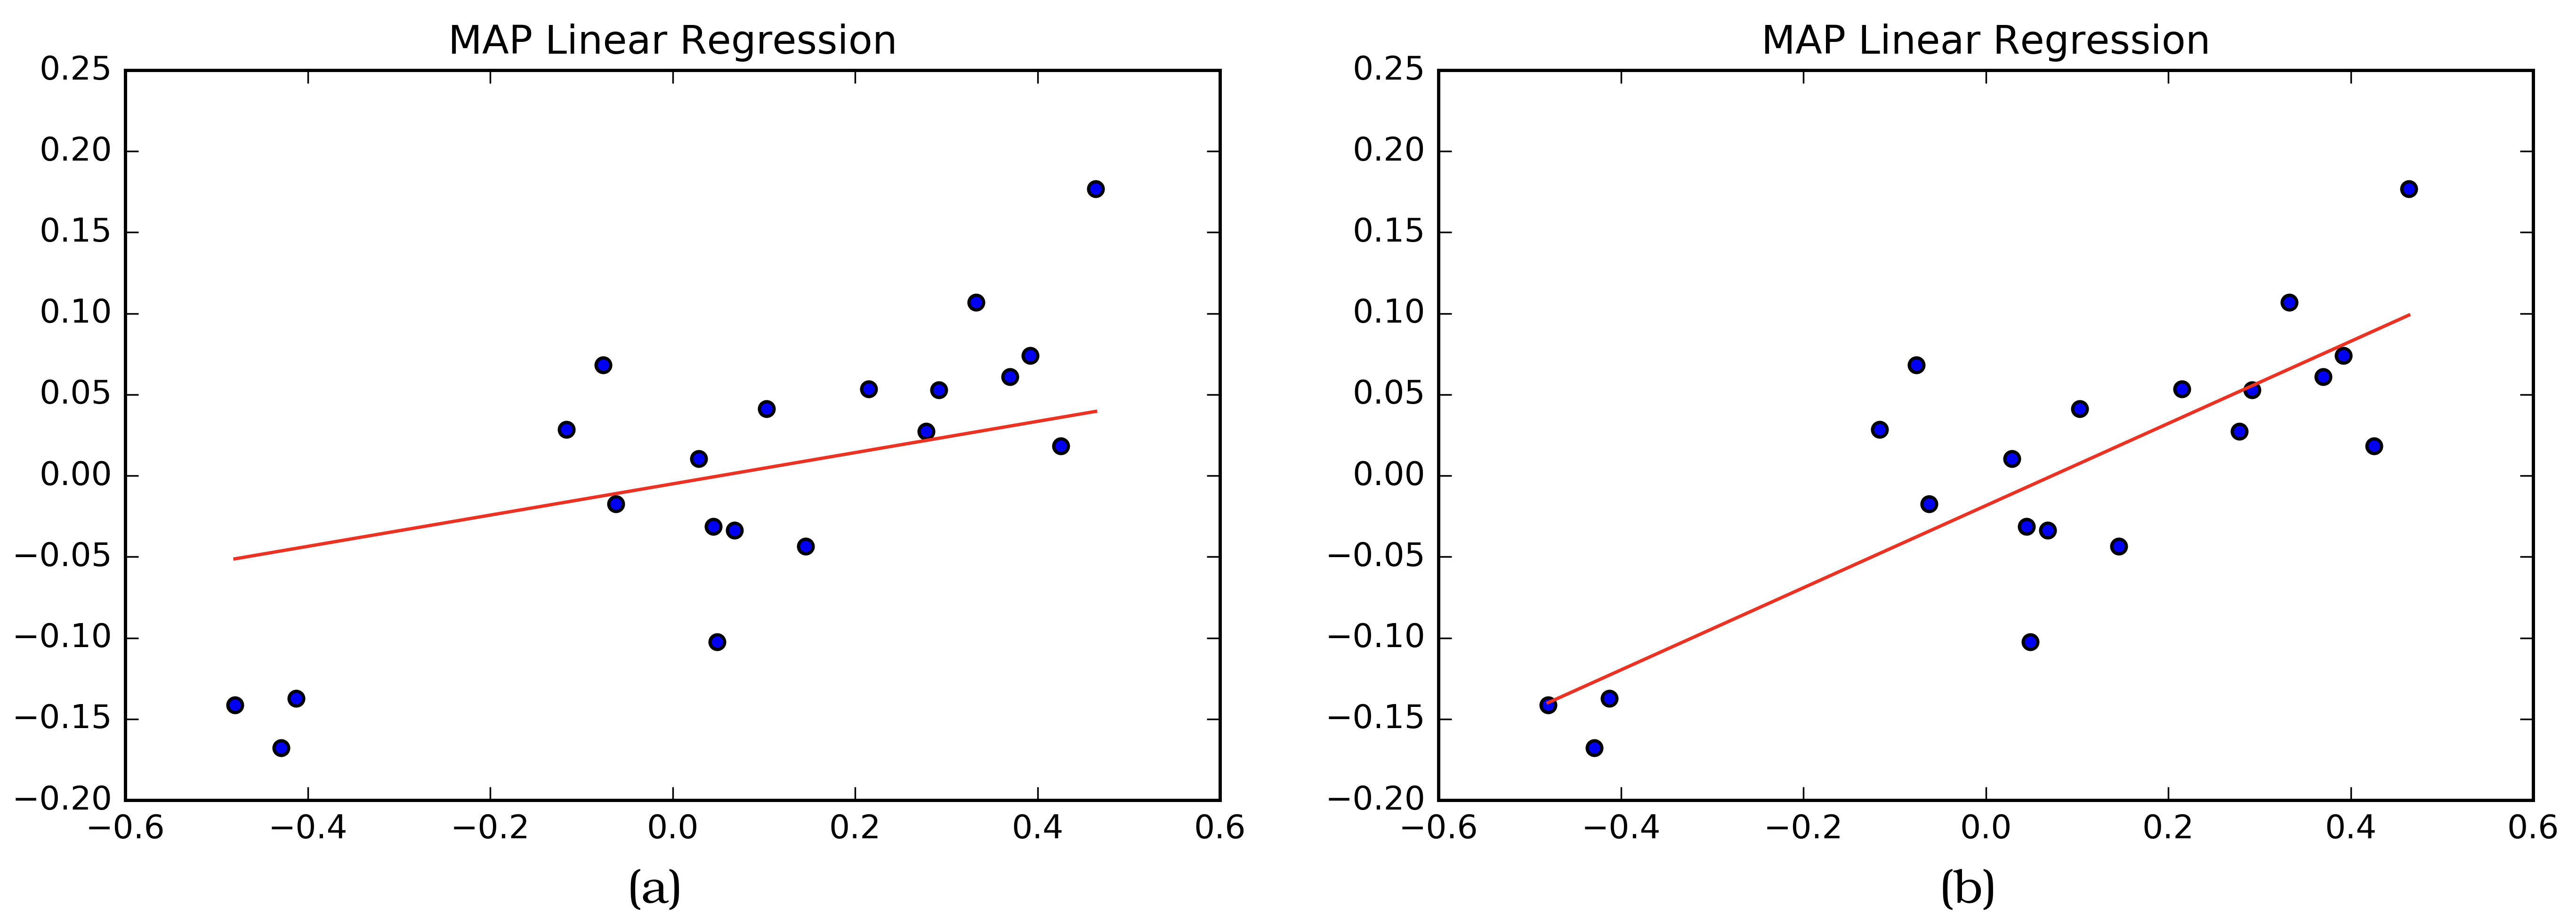
\includegraphics[width=1\textwidth]{lin-map-combined}
    \caption{Linear regression with MAP estimation of the parameter $\boldsymbol\phi$. (a) has a small prior covariance of 0.001 whereas (b) has a larger prior of 0.8. The prior influences the fitting of the curve.}
  \label{fig:lin-map-combined}
\end{figure}



%%%%%%%%%%%%
\section{Non-Linear Regression} \label{sec:discussion}
%%%%%%%%%%%%
Linear Regression is useful when we expect our data and the targets to be nearly, if not perfectly, linearly related. However, this is usually not the case in real life, where we would more likely to expect a non-linear relationship between them.

This can be done by keeping the underlying Mathematics of linear regression, but extend to more general functions through transforming each data point with some non-linear basis function.

If we used linear regression on a non-linear dataset, the model becomes over-confident and over-estimate the target. Often, not all features of each datapoint is neccessarily useful in creating the model, making the model unncessarily complicated.

Let us examine how this would work with a polynomial transformation using Maximum Likelihood as an example.

\subsection{Using ML and Polynomial Transformation to Achieve Non-Linear Regression}
\begin{equation} \label{eq:non-lin-transformation}
    \begin{aligned}
        \mathbf{z}_i &= \mathbf{f} \left [ \mathbf{x}_i  \right ]
        \\
        &= 
        \begin{bmatrix}
            1 \\
            x_i \\
            x_i^2 \\
            x_i^3
        \end{bmatrix}
    \end{aligned}
\end{equation}

Mathematically, non-linear regression with ML is performed in a similar fashion as linear regression. We first perform non-linear transformation, such as polynomial transformation by applying a function to each data vector. An example is illustrated in \autoref{eq:non-lin-transformation}, where we are transforming each data vector to the third order.

\begin{figure}
  \centering
  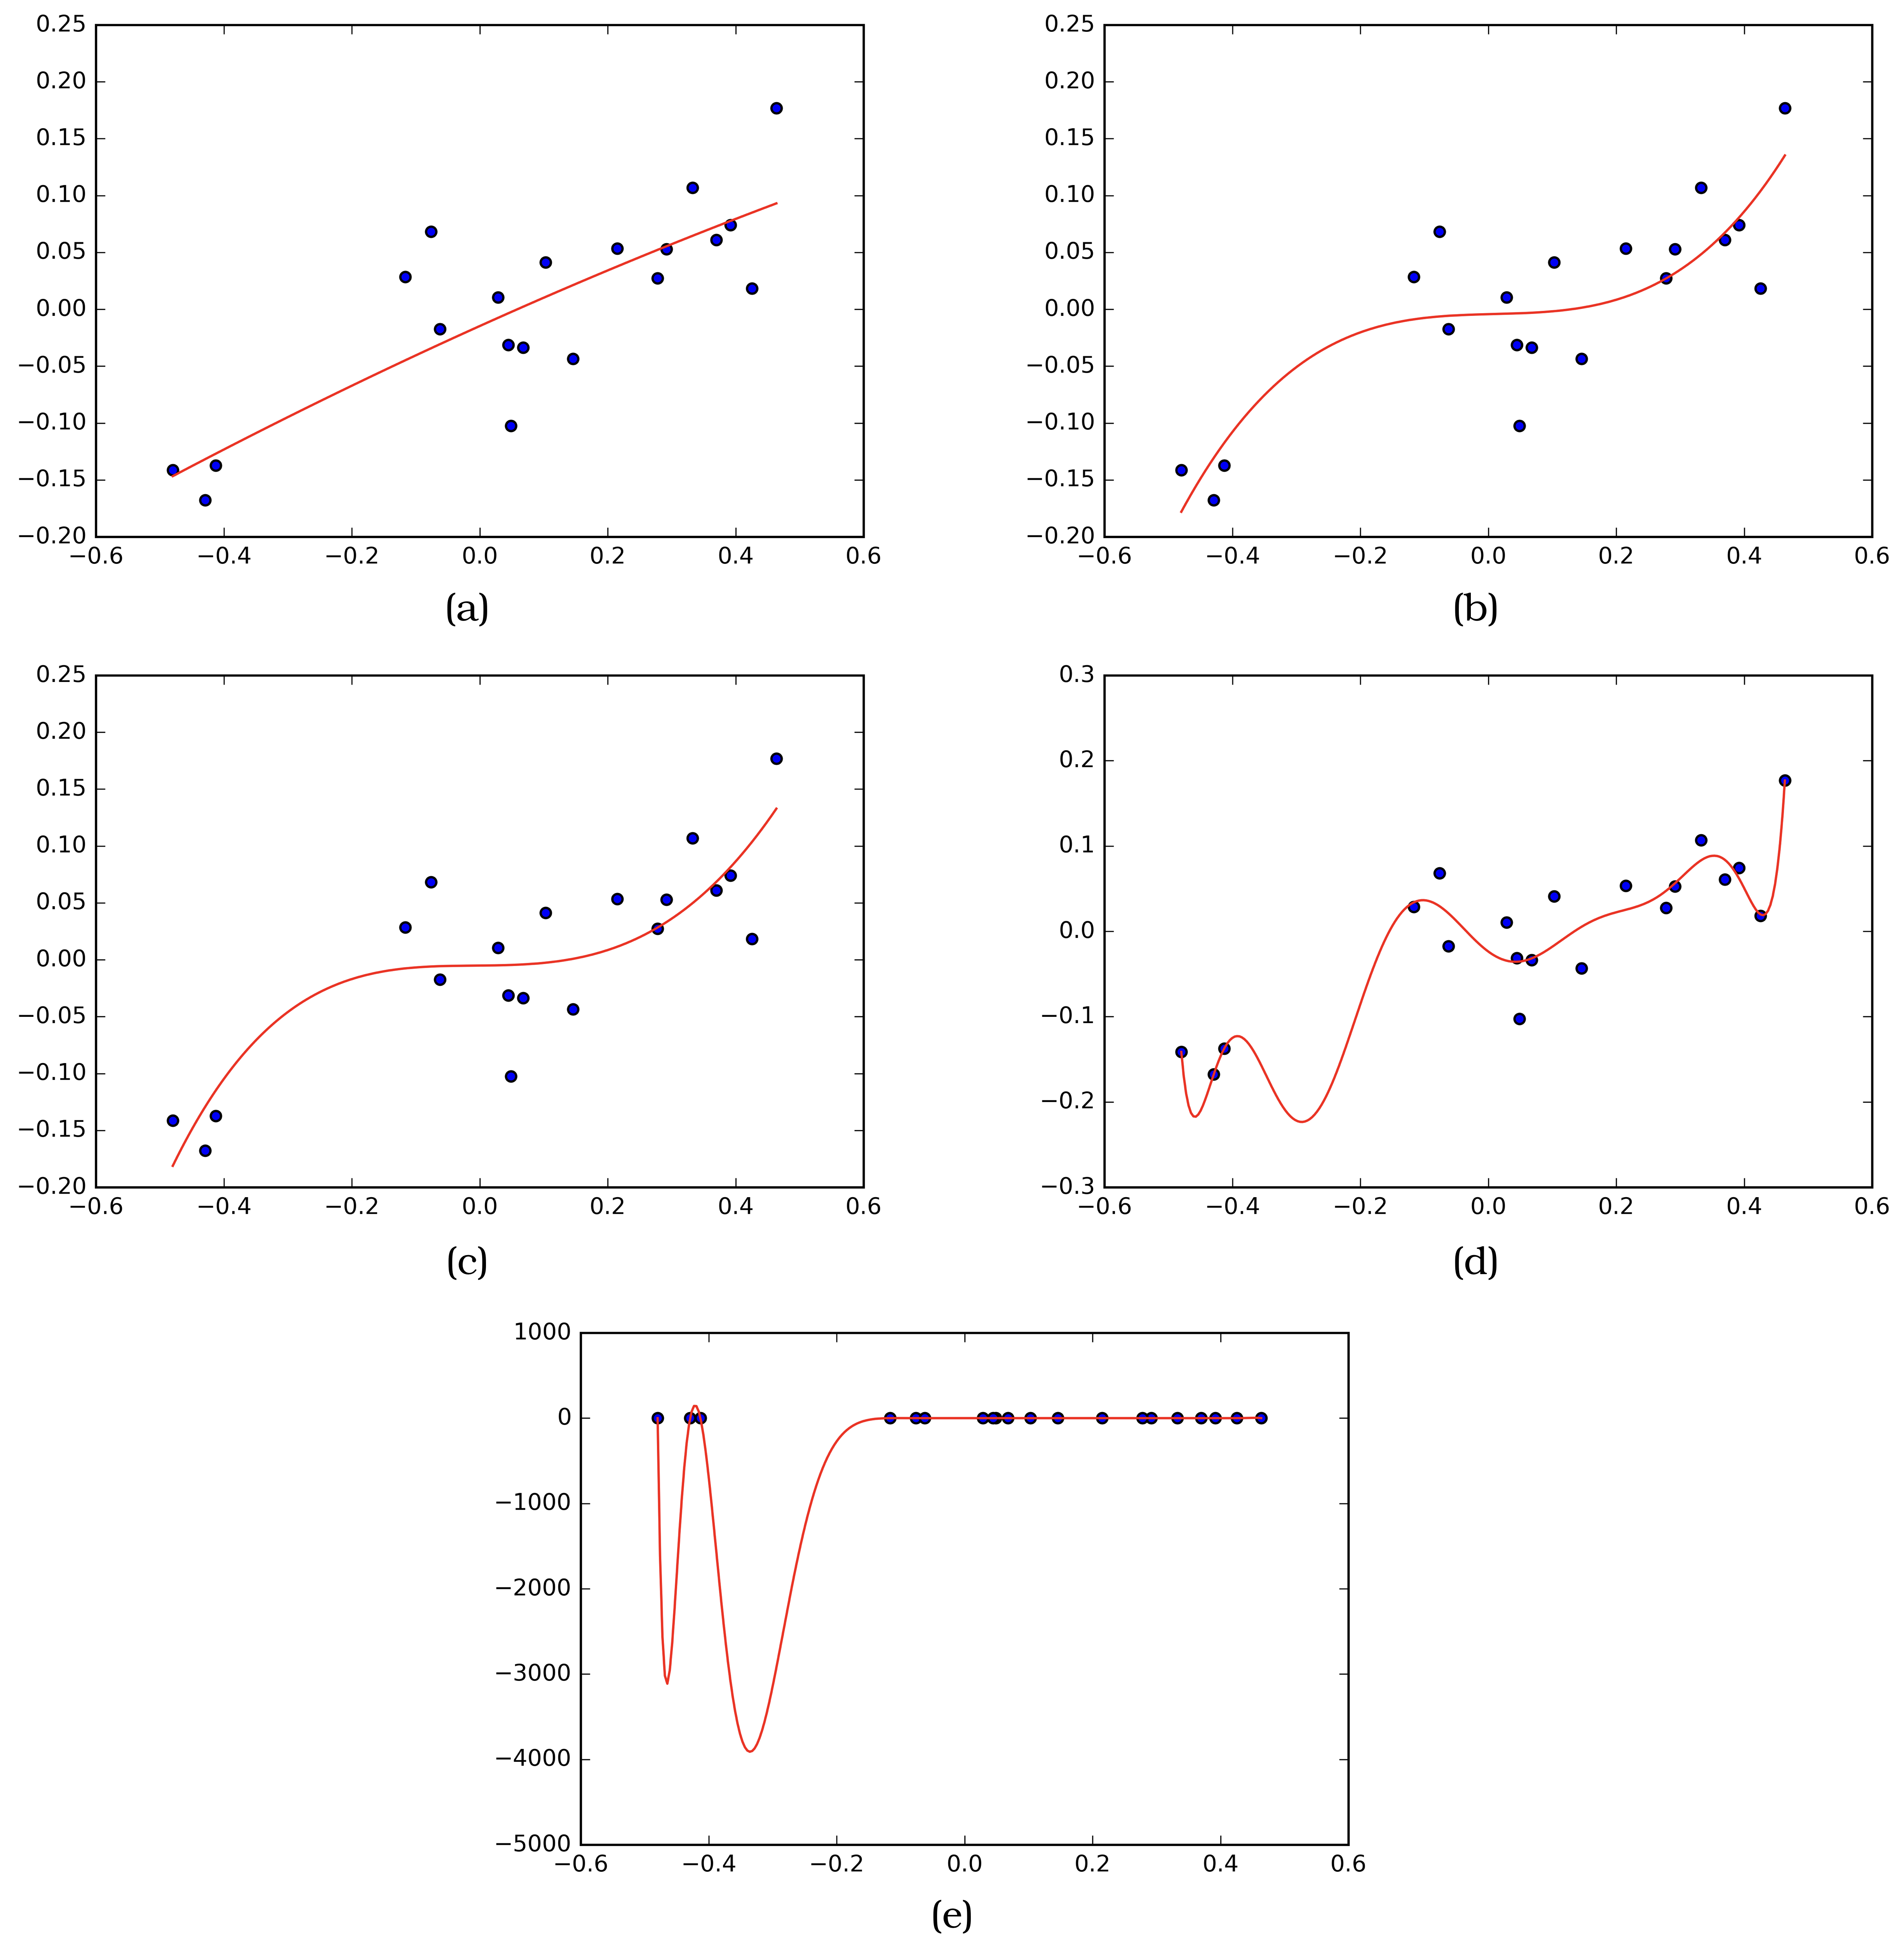
\includegraphics[width=1\textwidth]{non-combined}
	\caption{We compare different degrees of polynomial transformation - (a) order 2, (b) order 3, (c) order 4, (d) order 10 and (e) order 20. We can see that the model is overfitted in the cases of orders 10 and 20.}
  \label{fig:non-combined}
\end{figure} 

By substituting $\mathbf{X}$ with the matrix of all transformed data vectors $\mathbf{Z}$ in the linear ML solution equations in \autoref{eq:ml-params}, we obtain the ML solutions to non-linear regression.

\subsection{Overfitting}
Choosing an appropriate of transformation order is crucial. If too high an order is chosen, the model would be fitted very closely to the training data, and risk to be overfitted. 

An overfitted model possess very little predictive power. When we ask such a model to provide a prediction on unseen data, it would struggle to provide an expected or reasonable value.

Consider some datapoints that is generated from a order 3 equation where we attempt to fit a non-linear model to in \autoref{fig:non-combined}. We can see that as the order goes much higer than the actual order of the training data that the model starts to overfit.

Notice in sub-figures (d) and (e) in \autoref{fig:non-combined}, the curve is fitted too closely to the training data, which disallows it to be generic enough to predict unseen data. It is most noticable in the gap between -0.4 to -0.15 in the x-axis that the model would predict poorly. Intuitively, we would not expect the world state (y-axis) prediction to vary rapidly, but rather, steadily going up, as seen in cases (b) and (c).

\textit{I was unable to debug my code generating the Bayesian Inferences heatmap-styled plot to show the probability distribution. However, I have made an attempt in computing and plotting it in the 'Bayesian Linear Regression' section in the attached iPython notebook (both notebook and HTML format).}

%%%%%%%%%%%%
% \begin{figure}[H]
  % \centering
  % 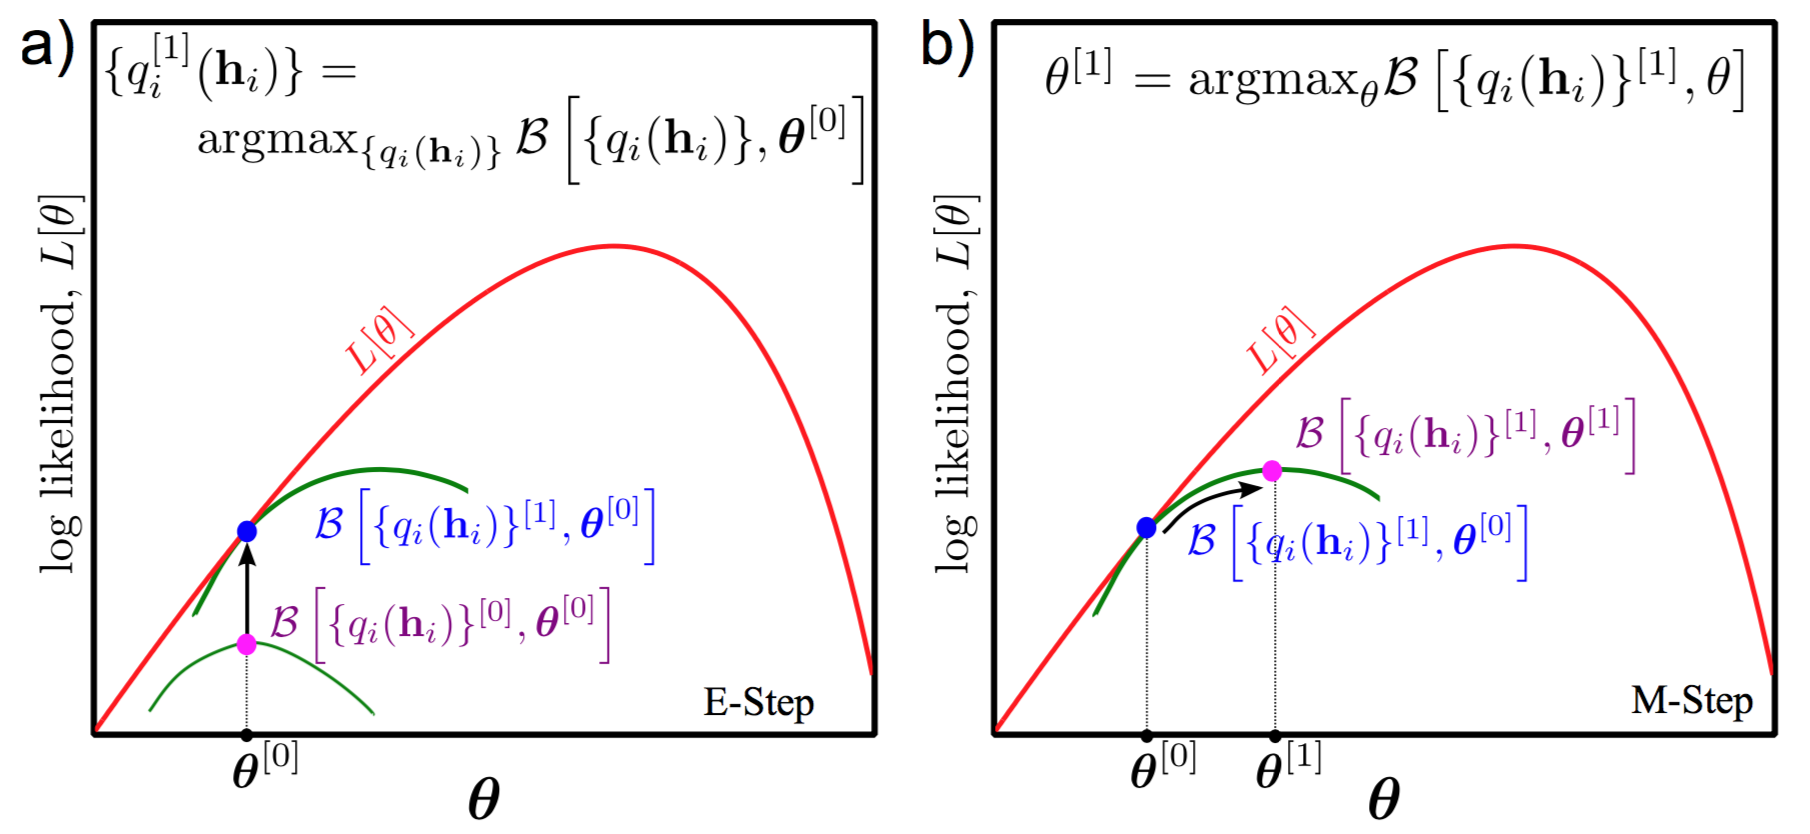
\includegraphics[width=0.7\textwidth]{em-overview}
    % \caption{(left) The graph shows an E-step, where manipulating the probability distributions changes all values of the lower bound for every $\boldsymbol{\theta}$, hence the whole curve moves towards the red curve, which is the actual log likelihood curve. (right) The graph shows an M-step, where the $\boldsymbol{\theta}$ is changed while fixing $q_{i}(\boldsymbol{h}_{i}$ to improve the estimate from the blue dot to the purple dot. (Figure taken from \cite{prince}.)}
  % \label{fig:em-overview}
% \end{figure} 

% \printbibliography

\end{document}
